% tikzpic.tex
\documentclass[crop,tikz]{standalone}% 'crop' is the default for v1.0, before it was 'preview'
\usetikzlibrary{calc}% tikz package already loaded by 'tikz' option

\usepackage{cmbright}
\usepackage[T1]{fontenc}

\usepackage{graphicx}

\begin{document}
\begin{tikzpicture}[x=1in,y=1in]
  \node[inner sep=0] at (4.25,5.5)
    {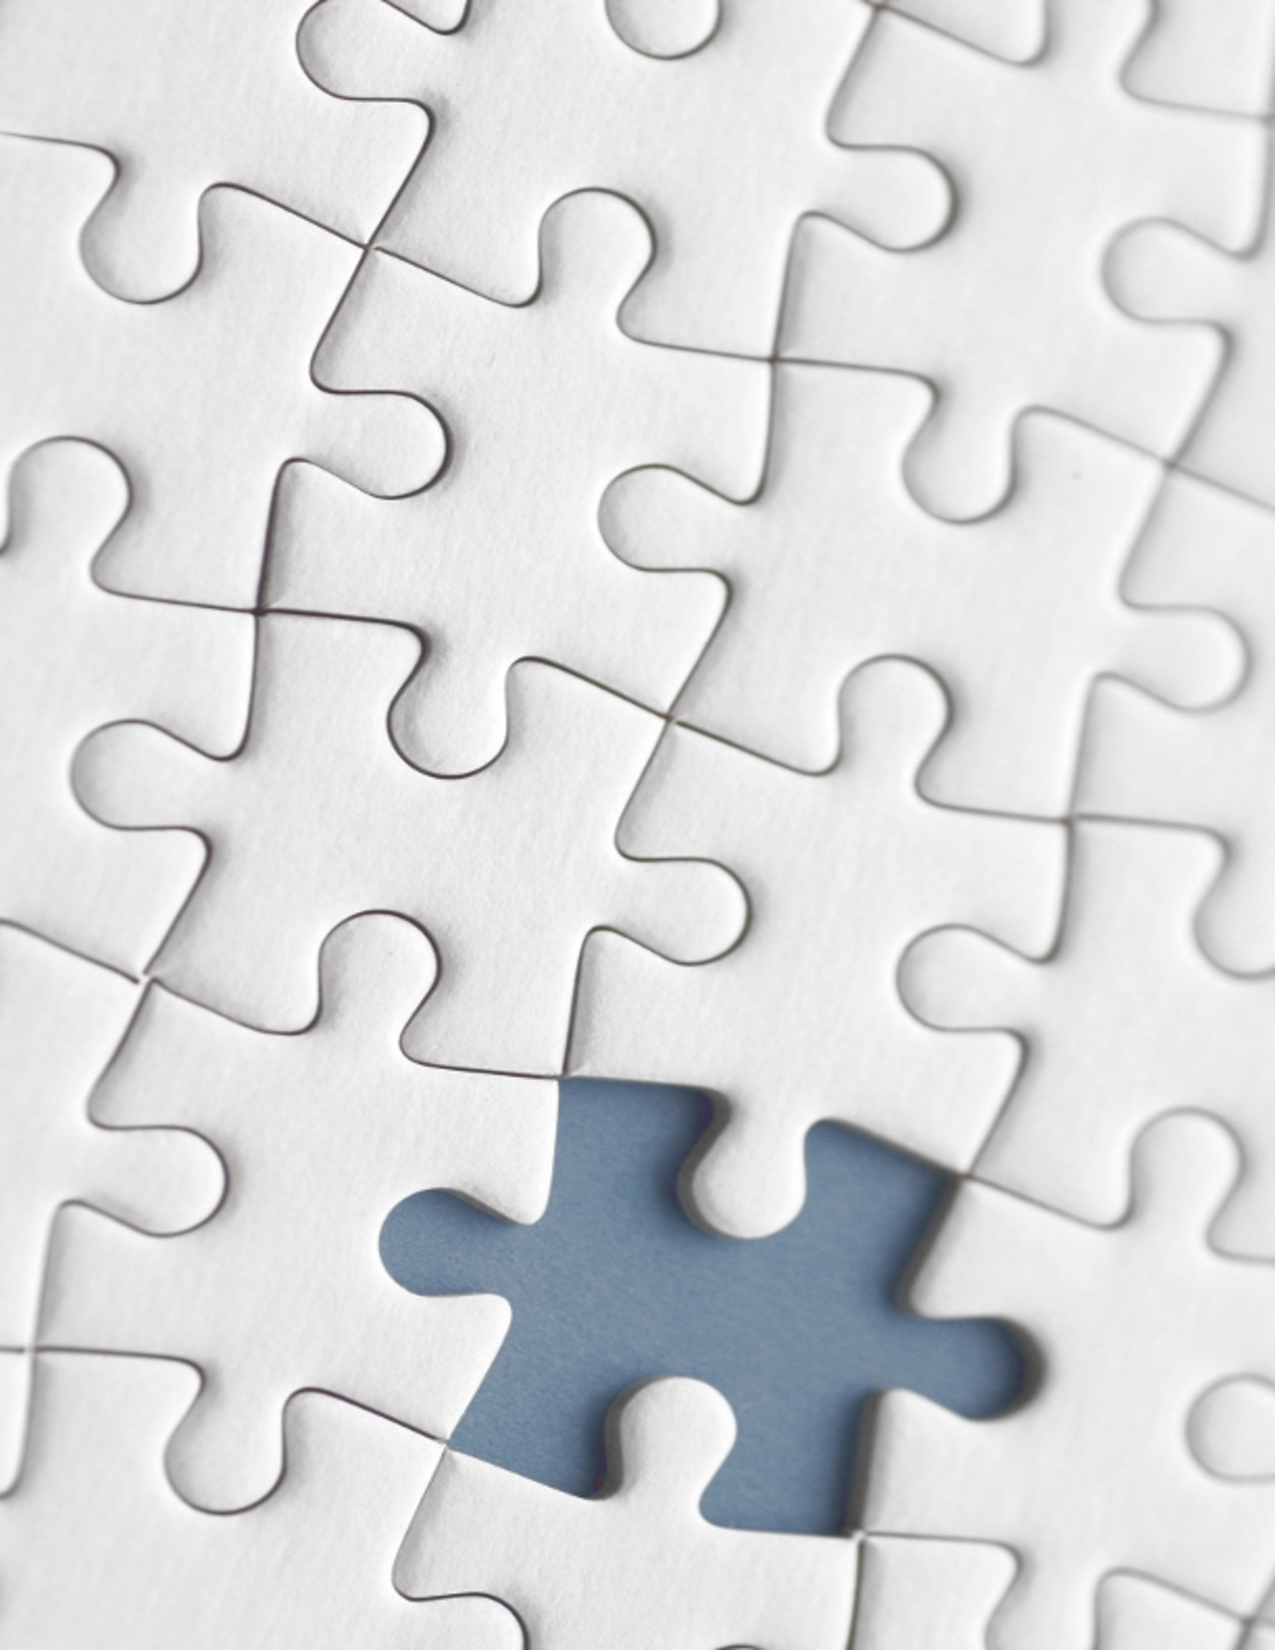
\includegraphics[width=8.5in]{puzzle-pieces.pdf}};

  \draw[fill=white,rounded corners] (1,7.5) rectangle +(6.5,2.5);
  \draw[fill=white,rounded corners] (1,4.25) rectangle +(6.5,2.75);
  \draw[fill=white,rounded corners] (1,1) rectangle +(6.5,2.5);



  \node[inner sep=0] at (4.25,9)
    {
\includegraphics[width=5in]{banner-color.pdf}};

  \node[inner sep=0] at (4.25,8)
    {\Huge\bf High School Challenge '17};



  \node[inner sep=0, align=center, rotate=15] at (3.5,6)
    {\bf\Large Nlx ftmaxftmbvte ikhuexf-lheobgz ldbeel mh \\\\
    \bf\Large ukxtd vhwxl tgw lheox inssexl! };

  \node[inner sep=0, align=center, rotate=15] at (5,5)
    {\bf\Large Use mathematical problem-solving skills to \\\\
    \bf\Large break codes and solve puzzles!};

  \node[inner sep=0] at (4.25,5.5)
    {\Large\(+7=\)};



  \node[inner sep=0] at (2.5,2.25)
    {
\includegraphics[height=1.3in]{south-alabama-logo.png}};

  \node[inner sep=0,align=center] at (5.25,2.25)
    {
      \Large Hosted by\\\Large\textbf{The University of South Alabama} \\
      \large on \textbf{2017 March 25} \\\\\\
      \large For teams of 9th-12th graders. \\
      \large Visit \textbf{MaPPmath.org} or contact \\
      \large Dr. Steven Clontz \(\langle\)sclontz@southalabama.edu\(\rangle\) \\
      \large for details!
    };


\end{tikzpicture}
\end{document}
